%    Documentation for PRU ADC Project
%    Copyright (C) 2016  Gregory Raven
%
%    This program is free software: you can redistribute it and/or modify
%    it under the terms of the GNU General Public License as published by
%    the Free Software Foundation, either version 3 of the License, or
%    (at your option) any later version.
%
%    This program is distributed in the hope that it will be useful,
%    but WITHOUT ANY WARRANTY; without even the implied warranty of
%    MERCHANTABILITY or FITNESS FOR A PARTICULAR PURPOSE.  See the
%    GNU General Public License for more details.
%
%    You should have received a copy of the GNU General Public License
%    along with this program.  If not, see <http://www.gnu.org/licenses/>.

\chapter{System Diagrams}

\begin{figure}[H]
	\centering
	\includegraphics[width=0.6\textwidth]{diagrams/system_diagram}
	\centering\bfseries
	\caption{Beagle Bone Green Wireless Irrigation Control System}
\end{figure}

The above diagram shows the main components of the system.  A reference section 
is included which has a complete parts list.


\section{GNU/Linux Operating System on Host ARM Processor}

The command uname -a on the BBG used to develop this project reports this:

\begin{verbatim}
Linux BBG2 4.4.30-ti-r64 #1 SMP Fri Nov 4 21:23:33 UTC 2016 armv7l GNU/Linux
\end{verbatim}

The latest IOT image has a newer kernel.  It is not a major update as of December 18, 2016.






